\documentclass{article}
\usepackage{natbib}
\usepackage{graphicx}
\graphicspath{{./images/}}

%opening
\title{Literatuurstudie: OZT 2018-2019}
\date{07/03/2019}
\author{Santi Meremans \\ Bono Opalfvens \\ Fé Vanmanshoven \\ Gautier de Bruijne \\\\ Hogeschool Gent \\ Toegepaste Informatica \\ Groep 19, Dhr. De Bruyne}

\begin{document}

\maketitle
\pagenumbering{gobble}
\newpage

\renewcommand*\contentsname{Inhoudstafel}

\tableofcontents
\newpage

\pagenumbering{arabic}
\section{Inleiding}
In het kader van onderzoekstechnieken hebben we verschillende artikels i.v.m. "Long term retention" onderzocht en vergeleken. Uit deze artikels hebben we de hoofdzaken geselecteert en samengevoegd in onze studie, zodat we de voor- en nadelen van de verschillende onderzoeken kunnen bekijken en tot een efficiënte manier van werken kunnen komen.
\\\\
Tevens hebben we deze artikels ook kritisch bekeken en zelf enkele onderzoeksvragen met bijhorende hypothesen opgesteld, die behandeld zouden kunnen worden.

\section{Conceptueel model}
\subsection{Onderzoeksvragen en hypothesen}
\begin{itemize}
	\item O1: Zijn er verschillen in resultaten bij het gebruik van een placebomiddel i.p.v. rilatine, bij studenten zonder ADHD?
	\begin{itemize}
		\item HO1: Een placebo-middel heeft minstens een even grote invloed op de prestaties van een student zonder ADHD, vergeleken met wanneer ze Rilatine genomen hebben.
		\item H02: Een placebo-middel heeft een kleine invloed op de prestaties van een student zonder ADHD, vergeleken met wanneer ze Rilatine genomen hebben.
		\item H03: Een placebo-middel heeft geen invloed op de prestaties van een student zonder ADHD, vergeleken met wanneer ze Rilatine genomen hebben.
	\end{itemize}
\begin{center}
	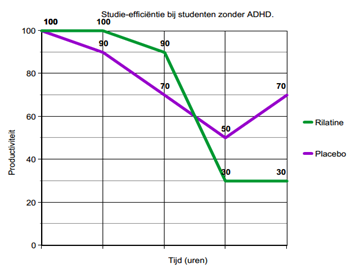
\includegraphics[width=8cm, height=5cm]{O1}
\end{center}
\newpage
	\item O2: Zijn er verschillen in resultaten bij het gebruik van een placebomiddel i.t.v. rilatine, bij studenten met ADHD?
	\begin{itemize}
		\item H01: Een placebo-middel heeft minstens een even grote invloed op de prestaties van een student zonder ADHD, vergeleken met wanneer ze Rilatine genomen hebben.
		\item H02: Een placebo-middel heeft een kleine invloed op de prestaties van een student zonder ADHD, vergeleken met wanneer ze Rilatine genomen hebben.
		\item H03: Een placebo-middel heeft geen invloed op de prestaties van een student zonder ADHD, vergeleken met wanneer ze Rilatine genomen hebben.
	\end{itemize}

\begin{center}
	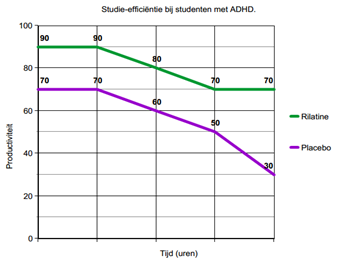
\includegraphics[width=8cm, height=5cm]{O2}
\end{center}
	\item O3: Is er een verband tussen de motivatie en/of eigen studiemethode en de resultaten van de student?
	\begin{itemize}
		\item H01: Er is geen verband tussen de motivatie en/of eigen studie methode en de resultaten van de student.
		\item 
		H02: Er is een verband tussen de motivatie en/of eigen studie methode en de resultaten van de student.
	\end{itemize}

\begin{center}
	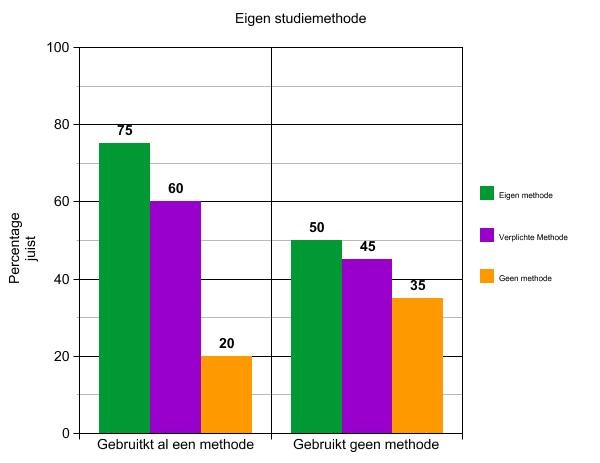
\includegraphics[width=8cm, height=5cm]{O3}
\end{center}
	\item O4: Is er een verband tussen de efficiënte van 'massed studie' en 'retrieval practice' en de complexiteitsgraad van het studiemateriaal?
	\begin{itemize}
		\item H01: Wanneer de graad van complexiteit stijgt wordt 'massed studie' efficiënter en 'retrieval practice' minder efficiënt.
		\item H02: Wanneer de graad van complexiteit stijgt wordt 'massed studie' minder effectief en 'retrieval practice' effectiever.
		
		\begin{center}
			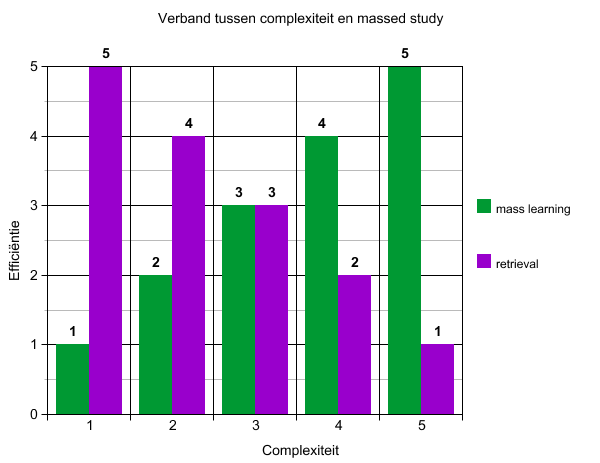
\includegraphics[width=5cm, height=3cm]{O4-H1}
			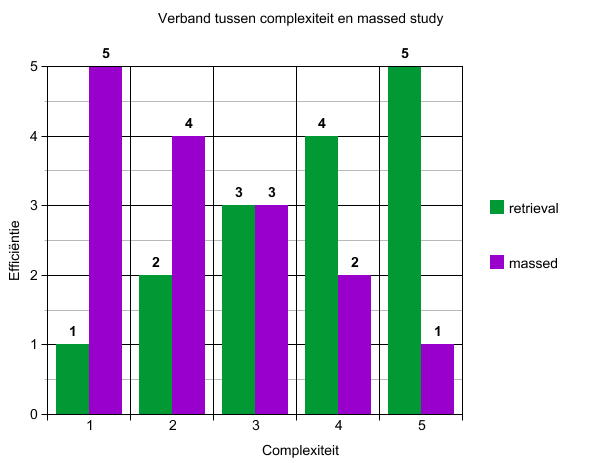
\includegraphics[width=5cm, height=3cm]{O4-H2}
		\end{center}
	\end{itemize}

\item O5: Wat is de tijdsbesteding voor 'elaborative practice' in tegenstelling tot 'retrieval practice'?
\begin{itemize}
\item H01: Deze methode neemt meer tijd in beslag dan gewoon 'retrieval practice'.
\item H02: Deze methode neemt minder tijd in beslag dan gewoon 'retrieval practice'.\\
\begin{center}
	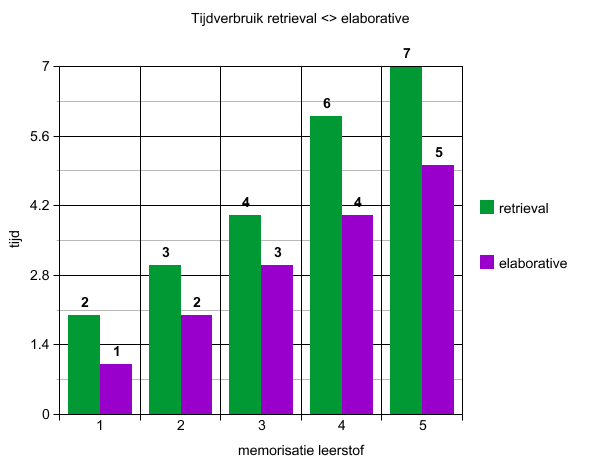
\includegraphics[width=5cm, height=3cm]{O5-H1}
	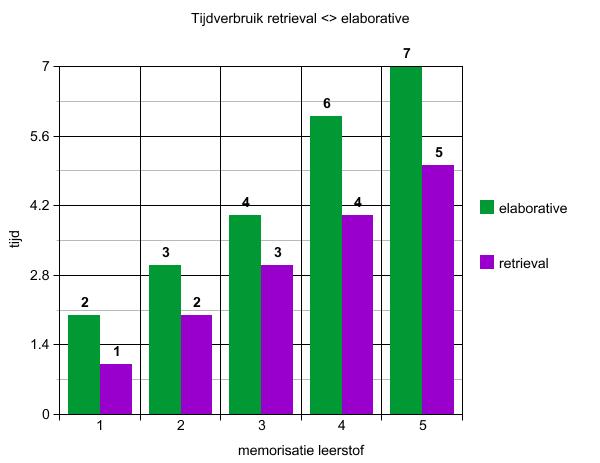
\includegraphics[width=5cm, height=3cm]{O5-H2}
\end{center}
\end{itemize}
\newpage
\item O6: Tot hoeveel iteraties blijft 'space learning' een efficiënte studiemethode?
\begin{itemize}
	\item H01: Na enkele iteraties daalt de efficiëntie van 'space learning'.
	\item H02: De efficiënte van 'space learning' blijft stabiel onafhankelijk van het aantal iteraties.
\end{itemize}
\begin{center}
	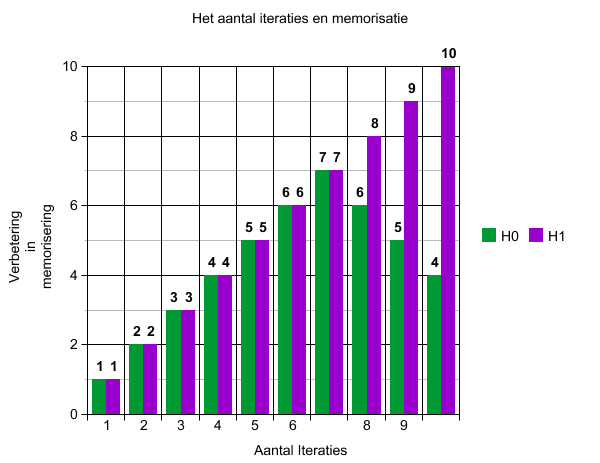
\includegraphics[width=8cm, height=5cm]{O6}
\end{center}
\end{itemize}

\newpage
\section{Literatuurstudie}
\subsection{Efficiënt studeren}


	Roedeger en Karpicke brengen ons bij dat leren kan op verschillende manieren met verschillende gevolgen. We bespreken verschillende studeermethoden met een duidelijke efficiëntie, invloed en duur van memorisatie. 
	\\
	We beginnen ons literatuuronderzoek te bespreken met als meetstaaf memorisatie. 2 technieken bleken zeer efficiënt uit verschillende onderzoeken.
	Jezelf overhoren behaalde de beste resultaten, dit is ook een van de meest onderzochte methoden.
	Dit kan bijvoorbeeld via oefentests, bijvoorbeeld een overhoring.
	\\\\
	Uit een experiment waarbij studenten enkele woorden uit het hoofd moesten leren bleek dat de groep die achteraf niet overhoord was slechts 4 procent van de gegeven woorden nog wist, bij de overhoorde groep bedraagde dit 35 procent. 
	\\\\
	In een ander experiment werd er de keuze gegeven om na het studeren van de woorden deze nogmaals te bekijken of overhoord te worden. De studenten die de woorden instudeerden via de overhoring wist nog 80 procent van de woorden, de andere slechts 36 procent. 
	Een mogelijke verklaring is dat oefentests intensiever het langetermijngeheugen stimuleren.
	\\\\
	Gespreid leren is ook een belangrijke factor om informatie voor een langdurige periode te onthouden.
	Uit een online studie blijkt dat voor het leren van triviale feitjes de beste resultaten werden behaald als de intervallen tussen de leerperioden ongeveer 10 tot 20 procent bedroeg.
	Dit zou willen zeggen dat wanneer iemand iets 1 jaar wilt memoriseren er een periode van 1 tot 2 en een halve maand tussen de studeerperiodes zouden moeten zitten. Uit onderzoek is gebleken dat wanneer men de leerstof over een periode kan spreiden gemiddeld 10 procent meer onthouden wordt.
	\\\\
	Ook is de feedback belangrijk, het zou bijvoorbeeld geen zin hebben om een test te maken om deze dan niet te verbeteren achteraf. Ook hier speelt tijd een grote rol. Zo zou het goed zijn om even te wachten met de oplossingen te geven. Omdat wanneer je dan verbeterd je de informatie terug opnieuw moet opnemen. Waardoor het geheugen getraind wordt om deze informatie op te halen.
	\\
	Maar de munt heeft ook een keerzijde, het zou ook kunnen dat wanneer je bijvoorbeeld veel fouten hebt gemaakt het beter is om de oplossing onmiddelijk te bekijken. Zodat je direct de foutief geleerde informatie kan identificeren en verbeteren.
	\\\\
	Deze onderzoekstechnieken werken en geven ook mooie resultaten af bij de steekproef. Maar wat bij andere onderwerpen? Deze onderzoeken gaan allemaal over niet-complexe onderwerpen, zoals triviale feitjes of memoriseren van een rij woorden. Maar wat met complexere onderwerpen? Zoals wiskunde of fysica? Hebben deze onderwerpen een andere aanpak nodig? Misschien kunnen we onze leermethode aanpassen aan het onderwerp? Misschien is een efficiënte manier om geschiedenis van buiten te leren een slechte manier om POD of wiskunde te leren. 
	\\\\
	We beginnen bij een methode die als het ware als een extensie fungeert voor spaced learning. Net zoals in spaced gaan we niet leren in 1 blok maar periodiek. Het verschil zit hem in de onderwerpen. In plaats van willekeurige onderwerpen te leren gaan we onderwerpen bewust kiezen voor bepaalde periodes, zodat er onderlinge samenhang is. Het logisch gevolg zou zijn dat er onderling linken worden gelegd waardoor je jezelf vragen zal stellen. hier komen we later op terug. Het artikel (Bjork \& Bjork) zegt dat spaced learning het best is om het memoriseren te bevorderen waarop de paper van Rawson zegt dat interleaved beter is om gecategoriseerd te leren.
	\\\\
	Het onderzoek op interleaved leren was hier wel negatief uitgedraaid, al vinden wij dat de steekproef weinig steek hield. Het was maar 1 en niet complex onderwerp. Het ging over soorten fobiën, men liet dan 1 fobie zien met 4 kenmerken (blocked) of men liet 4 fobiën zien met 1 sleutelkenmerk die bij alle 4 pastte (interleaved). Wij zouden graag interleaved onderzoeken maar niet met 1 onderwerp. Wij zouden bijvoorbeeld wiskunde en fysica afwisselend combineren. Bijv 50 min fysica kwartier pauze 50 min wiskunde. Zo zou men miss inzicht kunnen verwerven in logische redeneringen aangezien je formules van de wiskunde soms kan implementeren in de fysica en omgekeerd.
	\\\\
	Wanneer dit getest en waargenomen is zouden we ook nog een combinatie willen maken met elaborative study. Onze paper van Megan Smith \& Yana Weinstein beweert om een onderwerp volledig te verstaan er connecties gemaakt moeten worden. Deze connecties kunnen in het dagelijks leven gebeuren (bijv begrijpen hoe iets werkt). Het stellen van vragen beweren ze, is vitaal om het gegeven volledig te begrijpen. Door jezelf vragen te stellen over het onderwerp zullen je dingen opvallen waar je nog niet eens over nagedacht zou hebben, verbanden zullen zich blootleggen.
	\\\\
	Ook weten we van grote mathematicussen dat zij ook vaak doorbraken hebben gemaakt door het stellen van vragen aan zichzelf. Daarom zou een mooie test zijn om een onderwerp te studeren met interleaved practice en daarna nog een klein reflectiemoment van wat er geleerd is.
	\\\\
	Na het bespreken van de “interne” factoren hebben we ook nog een externe factor erbij genomen die past in het tijdskader anno 2019. We hebben er een onderzoek bij genomen van ....
	In dit onderzoek ondernamen ze een kwalitatieve beoordeling van attitudes ten aanzien van cognitieve verbetering - het gebruik van farmaceutische medicijnen om het normale functioneren van de hersenen te verbeteren. Ze hebben dit getest door 19 (14 vrouwen en 5 mannen) semigestructureerde interviews met Australische universiteitsstudenten te houden. 
	\\\\
	De meeste studenten beschouwden cognitieve verbetering als onacceptabel, deels omdat ze dachten dat het onethisch was, maar er was een gebrek aan consensus over de vraag of het vergelijkbaar was of verschilt van het gebruik van steroïden in de sport. 
	Het debat heeft zich gericht op de vraag of het eerlijk en ethisch is om voorgeschreven stimulerende middelen te gebruiken voor verbeterde concentratie. Studies met Canadese studenten hebben aangetoond dat veel mensen cognitieve verbetering identificeren als een vorm van valsspelen omdat het een oneerlijk voordeel oplevert. Studenten hebben ook hun bezorgdheid uitgesproken over het feit dat wijd verspreid gebruik van geneesmiddelen voor cognitieve verbetering anderen kan dwingen om zich met het gedrag bezig te houden en dat een verhoogd gebruik indirecte druk zal leggen op niet-gebruikers om cognitieve versterkers te nemen om te voorkomen dat ze achtergesteld raken. Ondanks de zorgen over oneerlijkheid en dwang, hebben kwalitatieve interviews met studenten geconstateerd dat ze het recht van een individu op vrije keuze om al dan niet medicijnen te gebruiken voor cognitieve verbetering sterk steunen.
	
	
\newpage
\section{Bibliografie}
\bibliography{ref}
\bibliographystyle{apalike}

\newpage
\citet{art1}\\
\citet{art2}\\
\citet{art3}\\
\citet{art4}\\
\citet{art5}\\
\citet{art6}\\
\citet{art7}\\
\citet{art8}\\
\end{document}


